\chapter{Equações de primeiro e segundo grau}

\section{Introdução}

Ao escrever problemas em linguagem matemática, geralmente utilizamos equações. Vejamos alguns exemplos:

\begin{texemplo}
A renda de uma família é a soma das rendas do pai (P), da mãe (M) e de uma filha (F). Sabe-se que a renda total é \textit{R$\$$  4.500,00} e somando a renda do pai e da mãe, obtém-se \textit{R$\$$  3.100,00}. Qual é a renda do filha ?

\textbf{Solução}: Escrevendo a renda como uma equação temos:

\equacao{$R = P + M + F$}

Sabemos que \textit{P + M} = \textit{R$\$$  3.100,00, }e R=\textit{ R$\$$  4.500,00}. Substituindo \textit{ P + M } e \textit{R} na equação, temos:

\equacao{$4500 = 3100 + F$}

Para que o lado esquerdo da \hyperref[eqc:4.2]{Eq. (2)} seja igual ao lado direito, \textit{F = 1.400 }\qedsymbol{}
\end{texemplo}

\begin{justify}
Na \hyperref[eqc:4.2]{Eq. (2)} temos uma equação com uma letra, cujo valor desconhecemos, mas que desejamos determinar. Chamamos esta letra de \textit{incógnita}.
\end{justify}

\begin{texemplo}
O perímetro de um quadrado mede \textit{12 cm. }Quanto mede cada lado?

\textbf{Solução}: Chamaremos de \textit{x} (\textit{incógnita}, a grandeza desconhecida) o lado do quadrado e escrevemos uma equação para o perímetro:

\equacao{$P = 4 \cdot x$}

Substituindo \textit{12} no lugar de \textit{P} obtemos uma equação com uma incógnita.

\textit{2 = 4 $ \cdot $  x}

Novamente temos uma equação com uma incógnita. É fácil verificar que o lado do quadrado mede \textit{x = 3 cm} \qedsymbol{}

\end{texemplo}

\begin{texemplo}
a) O dobro de um número mais \textit{3} é igual a \textit{5}. Que número é esse?

b) O dobro de um número mais \textit{3} é igual a \textit{6}. Que número é esse?

\textbf{Solução}: a) Chamando esse número de \textit{x}, podemos escrever:

\equacao{$2x + 3 = 5$}

Novamente temos uma equação com uma incógnita. Para que o lado esquerdo da \hyperref[eqc:4.4]{Eq. (4)} seja igual ao lado direito, \textit{x = 1. }

b) Com o mesmo procedimento do item (a), podemos escrever:

\equacao{$2x + 3 = 6$}

\begin{justify}
A solução nesse caso, não é tão óbvia. Neste capítulo vamos estudar operações algébricas para encontrar o valor da incógnita de equações algébricas. A solução é \textit{x = 3/2}. Substitua esse valor de \textit{x} na equação dada e verifique se ambos os lados da equação são iguais \qedsymbol{}
\end{justify}

\end{texemplo}

Podemos elaborar equações de vários tipos:

\begin{multicols}{2}
\textit{3 $ \cdot $  (5+8) = 10+ 29}

\( 2+3x+x^{2}+5x^{3}+x^{4}=0 \)

\( \frac{1}{1+x^{2}}=0 \)

\( 3^{x+1}=2 \)

(Equação numérica)

(Equação polinomial de 4º grau)

(Equação racional)

(Equação exponencial)
\end{multicols}

Neste capítulo vamos estudar as soluções das equações polinomiais de 1º e 2º Grau.

\section{Solução da equação}

O(s) valor(es) da incógnita que torna ambos os lados iguais~é a  solução de uma equação. Para resolver equações é necessário conhecer suas propriedades.

\textbf{Propriedade fundamental das equações}:

\begin{caixa}
Se em ambos os lados da equação for realizada a mesma operação, a equação permanece verdadeira (é mantida a identidade da equação).
\end{caixa}

\begin{texemplo}
Consideremos uma equação numérica:   \textit{5 = 5}.

Evidentemente é uma equação verdadeira pois 5 é igual a 5!

\begin{enumerate}
\item Se adicionarmos +10 em ambos os lados, temos

+10 + 5 = 5 + 10

+15 = +15. A identidade foi mantida.

	\item Se adicionarmos -10 em ambos os lados, temos

-10 + 5 = 5 + (-10)

-5 = -5. A identidade foi mantida.

	\item Se multiplicarmos por 7 em ambos os lados, temos

7 $ \cdot $  5 = 5 $ \cdot $  7

\begin{enumerate}
	\item = 35. A identidade foi mantida.
\end{enumerate}

	\item Se dividirmos por 4 em ambos os lados, temos
\end{enumerate}

\( \frac{5}{4}=\frac{5}{4} \). A identidade foi mantida\qedsymbol{}
\end{texemplo}

\begin{texemplo}
Dada a equação \textit{3x = 2x + 5}, determine o valor de \textit{x}.

\textbf{Solução}: Usando a propriedade fundamental, se adicionarmos \textit{-2x} em ambos os lados da equação dada, temos:

\textit{-2x +3x = 2x + 5 - 2x}

\textit{x = 5}\qedsymbol{}
\end{texemplo}

Para resolver uma equação, precisamos isolar a incógnita em um dos lados. Os \textit{princípios aditivo} e \textit{multiplicativo} derivam da propriedade fundamental e a tornam mais prática.

\begin{caixa}
\textbf{Princípio aditivo}

Adicionando constantes ou variáveis em ambos os lados, a solução da equação permanece a mesma.
\end{caixa}

\begin{texemplo}
Dada a equação \textit{2x = x + 12}, determine o valor de \textit{x}.

\textbf{Solução}: Observemos que a solução é \textit{x = 12}. Precisamos reunir as expressões que contem \textit{x} em um lado da equação. Adicionando \textit{-x} em ambos os lados, obtemos:

\textit{-x +2x = x - x + 12}

\textit{x = 12}. Observemos que a solução permaneceu a mesma \textit{x = 12}~  \qedsymbol{}
\end{texemplo}

\begin{caixa}
\textbf{Princípio multiplicativo}
Multiplicando (ou dividindo) ambos os lados por constantes ou variáveis (diferente de zero), a solução da equação permanece a mesma.
\end{caixa}

\begin{texemplo}
Dada a equação \textit{2x = - 12}, determine o valor de \textit{x}.

\textbf{Solução}: Observemos que a solução é \textit{x = -6}. Multiplicando ambos os lados por $\frac{1}{2}$, obtemos:

 \( \frac{1}{2} \cdot 2x= -12  \cdot  \frac{1}{2} \)

\textit{x = -6}. Observemos que a solução permaneceu a mesma, \textit{x = -6} \qedsymbol{}
\end{texemplo}

\section{Equação do 1º Grau}

As equações polinomiais têm a forma de polinômios de uma incógnita igualados a zero:

\equacao{$a_{0}+a_{1}x+a_{2}x^{2}+a_{3}x^{3}+a_{4}x^{4}+ \ldots +a_{n}x^{n}=0$}

O grau de uma equação polinomial é o grau do maior expoente da incógnita. Assim,\textbf{ }

 \( 2+3x=0 \) ~~~ é uma equação de 1º grau

 \( 4+5x+x^{2}=0 \) ~ é uma equação do 2º grau

 \( 3+2x+x^{2}+5x^{3}+2x^{4}=0 \) ~ é uma equação do 4º grau e assim por diante.

\begin{tdefinicao}
A equação do 1º Grau tem a forma

\equacao{$ax + b = 0$}

Onde \textit{a} e \textit{b} são números reais e \textit{x} é uma incógnita.
\end{tdefinicao}

\begin{texemplo}
Mostre que a equação \textit{x + 3x +3(x-1) = 5} pode ser reduzida à forma

\textit{ax + b = 0}.

\textbf{Solução}: Multiplicando a constante \textit{3} pelo conteúdo do parêntesis, temos:

\textit{x + 3x +3x -3 = 5. }Adicionando os termos semelhantes e adicionando\textit{ +3} em ambos os lados da equação, temos:

\textit{7x -3+3 = 5+3}ou\textit{ }adicionando\textit{ (-8), }temos:

\textit{7x - 8 = 0. }Portanto, a equação dada é do 1º Grau\textit{~~ }\qedsymbol{}
\end{texemplo}

\begin{texemplo}
Mostre que a equação \( \frac{x-3}{2}=\frac{x+3}{3}+3 \) pode ser reduzida à forma

\textit{ax + b = 0} e resolva a equação.

\textbf{Solução}: Multiplicando toda equação por \textit{6}, temos:

 \[ 6 \left( \frac{x-3}{2} \right) =6 \left( \frac{x+3}{3}+3 \right) ~~~  \]

Efetivando os produtos, temos:

 \( 3x-9=2x+6+18~~~  \) \textit{.} Adicionando \textit{-2x} e \textit{-24} em ambos os lados, temos:

\textit{x - 33 = 0}. Portanto, a equação dada é do 1º Grau.

Para resolver a equação, basta adicionar \textit{+3}3 em ambos os lados.

\textit{x = 33} \qedsymbol{}
\end{texemplo}

\begin{caixa}
\textbf{Observemos que nas equações de 1º Grau existe apenas uma solução.}
\end{caixa}

\begin{exercicios}
	\exitem{Uma estratégia para resolver equações fracionárias de apenas um termo em cada lado da igualdade é multiplicando os meios e os extremos (lembrar de proporções):}

Se \( \frac{a}{b}=\frac{c}{d} \) então  \textit{a $ \cdot $  d = b $ \cdot $  c. }(\textit{a }e \textit{d }são os extremos e\textit{ b }e\textit{ c }são os meios)

\begin{enumerate}[label=\alph*)]
	\item Use essaestratégia~para~resolver~a~equação \( \frac{x}{2}=\frac{2}{3} \)

	\item A estratégia poderia ser usada para resolver~~   \( \frac{x}{2}=\frac{2x}{3}+\frac{1}{2} \) ~ ?
\end{enumerate}

	\exitem{Resolva a~equação \( \frac{x+1}{4}=x+\frac{1}{2} \) ~~~ :}

\begin{enumerate}
	\item Multiplicando ambos os lados pelo MMC dos denominadores

	\item Adicionando os termos do lado direito e igualando o produto dos meios e dos extremos.
\end{enumerate}

\exitem{Determine a solução das equações:}

\begin{enumerate}
	\item  \( x + 3 = 1 \)

	\item  \( 3x-3=x+1 \)

	\item  \( 3 \left( x+2 \right) =9 \)

	\item  \( 2 \left( 3x+3 \right) =3x \)

	\item  \( 2 \left( x-2x \right) =4 \left( x-1 \right)   \)

	\item  \( \frac{x-1}{2}=\frac{x-4}{3} \)

	\item  \( \frac{x+5}{4}=\frac{3x+3}{6} \)

	\item  \( \frac{12}{x}=\frac{3}{x}+\frac{3}{2} \)

	\item  \( 3 \left( x+5 \right) =\frac{x-20}{2} \)

	\item  \( \frac{1}{2}=\frac{x-2}{3} \)
\end{enumerate}

	\exitem{Resolva a equação  \( \frac{x}{5}+\frac{x-1}{10}=\frac{1}{2} \)  :}

\begin{enumerate}
	\item Adicionando as frações do lado esquerdo e depois resolvendo para \textit{x};

	\item Multiplicando toda a equação pelo MMC dos denominadores e depois resolvendo para \textit{x}.
\end{enumerate}

	\exitem{Resolva as equações:}

\begin{enumerate}
	\item  \( \frac{x}{3}+\frac{x-1}{2}=\frac{1}{3} \) { b)  \( \frac{1}{2}=\frac{x}{5}+2x~  \) c)  \( \frac{x}{2}+\frac{2x}{3}=\frac{1}{6} \) }
\end{enumerate}

 \((d)  \frac{x+1}{2}+\frac{3x}{4}=\frac{5x}{2} \) { e)~  \( \frac{5}{x+1}=\frac{3}{x+2}~  \) f)  \( \frac{1}{x+1}=\frac{2}{x+1}+\frac{1}{2} \) }

	\exitem{Determine:}

\begin{enumerate}
	\item Um número mais sua metade e mais 5 é 8. Que número é este?

	\item Um número mais sua metade e mais 5 é 3. Que número é este?

	\item A terça parte de um número, mais a metade desse número menos 1 é 1/3. Que número é este?
\end{enumerate}

	\exitem{O lado de um quadrado mede  \( x+2 cm \) , onde x é uma variável real. Qual é o valor de x, sabendo-se que o perímetro é 12 cm?}

	\exitem{A largura e o comprimento de um retângulo medem  \( xcm \)  e  \(  \left( x+3 \right) cm \) , respectivamente. Qual é o valor de \textit{x}, para que o perímetro seja:}

\begin{enumerate}
	\item P = 10 cm

	\item P = 12 cm
\end{enumerate}

	\exitem{A largura de um retângulo é dada pela expressão 3x$-$ 1 e o comprimento por  \( x+\frac{1}{2}. \)  Qual é o valor de \textit{x}, se a largura é a metade do comprimento?}

	\exitem{O comprimento de um campo de futebol é 30m maior do que a largura. Quais são as dimensões do campo, se o perímetro é 340m?}

	\exitem{Os lados, em sequência, de um triângulo diferem entre si por \textit{2 cm}. Quanto mede cada lado se o perímetro é 12 cm?}
\end{exercicios}

\section{Equação do 2º Grau}

\begin{caixa}
\begin{tdefinicao}
as equações de segundo grau têm a forma
\equacao{$a_{0}+a_{1}x+a_{2}x^{2}=0$, para $a_{2} \neq 0$\qedsymbol{}}
\end{tdefinicao}
\end{caixa}

\subsection{Solução da equação do 2º Grau incompleta}

Se ~ \textit{a\textsubscript{0}} ~ e/ou ~ \textit{a\textsubscript{1}}~~~ forem iguais a zero, a solução da \hyperref[eqc:4.8]{Eq. (8)} pode ser obtida facilmente usando a propriedade fundamental das equações. Vejamos os casos 1, 2 e 3:

\textbf{Caso 1}: Se \textit{a\textsubscript{0~ }= a\textsubscript{1~ }=~0. }Nesse caso a \hyperref[eqc:4.8]{Eq. (8)} tem a forma:

 \[ a_{2}x^{2}=0 \]

e a única solução é \textit{x = 0} \qedsymbol{}

\textbf{Caso 2}:  \textit{a\textsubscript{0~ }$ \neq $ ~0~  }e~~ \textit{a\textsubscript{1 }=~0. }Nesse caso a \hyperref[eqc:4.8]{Eq. (8)} tem a forma:

\equacao{\( a_{0}+a_{2}x^{2}=0 \).}

Adicionando (\textit{-a\textsubscript{0}}) em ambos os lados, temos:

\equacao{\( a_{2}x^{2}=-a_{0} \)}

Dividindo a \hyperref[eqc:4.10]{Eq. (10)} por \textit{a\textsubscript{2}} e em seguida aplicando raiz quadrada em ambos os lados, temos:

\equacao{\( x= \pm  \sqrt[]{-\frac{a_{0}}{a_{2}}} \).}

Como a raiz quadrada de números negativos não é número real (é número complexo), podemos afirmar que \textit{x} será real, somente se

\equacao{\( -\frac{a_{0}}{a_{2}} \geq 0 \) \qedsymbol{}}

\textbf{Caso 3}:~ \textit{a\textsubscript{1 }$ \neq $ ~0~  }e~ \textit{a\textsubscript{0}} \textit{=~0. }Nesse caso a \hyperref[eqc:4.8]{Eq. (8)} tem a forma:

\equacao{\( a_{1}x+a_{2}x^{2}=0 \).}

Colocando o fator comum \textit{x} em evidência, temos:

\equacao{\( x \cdot  \left( a_{1}+a_{2}x \right) =0 \)}

Esse produto de dois termos será zero somente \textbf{se um ou os dois termos} forem nulos. Assim, teremos duas soluções possíveis: \textit{x\textsubscript{1}} e \textit{x\textsubscript{2}}.

\begin{enumerate}
	\item \textit{x\textsubscript{1} = 0}~~~~~ ou

	\item  \( a_{1}+a_{2}x_{2} =0 \). Resolvendo para \textit{x}, temos:
\end{enumerate}

 \[  \]  \[ x =-\frac{a_{1}}{a_{2}} \]

A solução da equação de 2º grau, nesse caso, é

 \[ x_{1}=0~~  \] ~~e~   \(   x_{2}=-\frac{a_{1}}{a_{2}} \). \qedsymbol{}

\subsection{Solução da Eq. do 2º grau completa}

Quando nenhum coeficiente da equação de segundo grau for nulo, a solução pode ser obtida por fatoração do trinômio, completando o quadrado perfeito. Lembremos que

\begin{figure}[H]
	\begin{Center}
		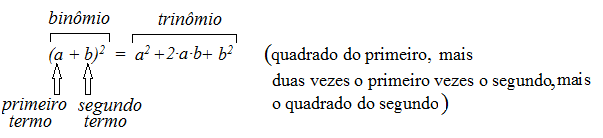
\includegraphics[width=5.91in,height=1.35in]{capitulos/equacoes_de_primeiro_e_segundo_grau/media/image2.png}
	\end{Center}
\end{figure}

Vejamos dois exemplos:

\begin{texemplo}
Determine as raízes da equação   \textit{x\textsuperscript{2} + 6x + 9 = 0}.

\textbf{Solução}: Nesse~caso, temos um TQP, pois  \textit{a = x}~ e \textit{b=3}. Portanto,

\textit{2ab = 2 $ \cdot $  x $ \cdot $ 3 = 6x}~~ que é igual ao termo intermediário do trinômio. Assim,

\textit{x\textsuperscript{2} + 6x + 9 = (x+3)\textsuperscript{2}=0}. Aplicando raiz quadrada em ambos os lados, temos:

\textit{x + 3 = 0}. Adicionando (-3) em ambos os lados, temos:

\textit{x = -3~~~ }~~é a raiz da equação dada  \qedsymbol{}
\end{texemplo}

\begin{texemplo}
Determine~as raízes da equação   \textit{x\textsuperscript{2} + 5x + 6 = 0}.

\textbf{Solução}: Nesse caso, NÃO temos um TQP, pois  se \textit{a = x}~ e  \( b=\sqrt[]{6} \) ~ não temos uma identidade, comparando com o termo intermediário do trinômio:

\textit{2ab  =  2 $ \cdot $  x $ \cdot $  \( \sqrt[]{6}~  \)  $ \neq $ ~ } \textit{5x}.

Para obter um trinômio, vamos usar \textit{a = x}~ e determinar \textit{b}, tal que

\textit{5x}~~=  \textit{2ab  =  2 $ \cdot $  x} \textit{$ \cdot $  b} ou

\textit{5}~ =\textit{  2 } \textit{$ \cdot $  b}

\textit{b}~ =\textit{ 5/2 }.

Adicionando \textit{b\textsuperscript{2} =(5/2)\textsuperscript{2}}~~ em ambos os lados da equação dada, obtemos:

 \( x^{2}+5x+ \left( \frac{5}{2} \right) ^{2}+6= \left( \frac{5}{2} \right) ^{2} \). Adicionando (\textit{-6}) em ambos os lados e reescrevendo, temos

 \( x^{2}+5x+ \left( \frac{5}{2} \right) ^{2}=\frac{1}{4} \). Fatorando o TQP obtido, temos:

 \(  \left( x+\frac{5}{2} \right) ^{2}=\frac{1}{4} \). Aplicando raiz quadrada em ambos os lados, temos:

 \( x+\frac{5}{2}= \pm \sqrt[]{\frac{1}{4}}= \pm \frac{1}{2} \). Adicionando (\textit{-5/2}) em ambos os lados e operando, temos:

 \( x= \pm \frac{1}{2}-\frac{5}{2} \) \textit{~~~ }. Finalmente, as soluções da equação dada são:

 \( x_{1}=-2  \) \textit{ ~ }~ e~~  \( x_{2}=-3  \) ~~~~~ \qedsymbol{}

\end{texemplo}

O processo desenvolvido no Ex. 5.2 pode ser generalizado da seguinte maneira:

Inicialmente, para evitar o uso de sub-índices, vamos usar \textit{A=a\textsubscript{2}~;  B=a\textsubscript{1} e C=a\textsubscript{0}}  e reescrever a  \hyperref[eqc:4.7]{Eq. (7)} :

\equacao{\textit{Ax\textsuperscript{2}~+ Bx  + C = 0}.}

Para que o coeficiente de \textit{x\textsuperscript{2}} seja \textit{1}, vamos dividir a \hyperref[eqc:4.8]{Eq. (8)} por \textit{A}.

\equacao{\( \frac{Ax^{2}+Bx+C}{A}=\frac{0}{A} \) \quad ~~~ou~   \( x^{2}+\frac{B}{A}x+\frac{C}{A}=0 \)}

Para obter o TQP, vamos usar \textit{a = x}~ e determinar \textit{b}, tal que:

 \( \frac{B}{A}x=2ab=2xb \) \textit{. }Então\textit{~~~  \( b=\frac{B}{2A} \) ~~ }.

Adicionando ( \( b^{2}= \left( \frac{B}{2A} \right) ^{2} \) ) em ambos os lados da \hyperref[eqc:4.16]{Eq. (16)}, temos

 \( x^{2}+\frac{B}{A}x+ \left( \frac{B}{2A} \right) ^{2}+\frac{C}{A}= \left( \frac{B}{2A} \right) ^{2} \). Fatorando o TQP obtido e adicionando (-C/A) em ambos os lados, temos:

 \(  \left( x+\frac{B}{2A} \right) ^{2}= \left( \frac{B}{2A} \right) ^{2}-\frac{C}{A} \). Operando o lado direito e aplicando raiz quadrada em ambos os lados, temos:

 \( x+\frac{B}{2A}=\sqrt[]{\frac{B^{2}-4AC}{4A^{2}}} \). Adicionando  \( -\frac{B}{2A}~  \) em ambos os lados, temos:

 \( x= \pm \sqrt[]{\frac{B^{2}-4AC}{4A^{2}}}-\frac{B}{2A} \) ~~~~ ou

\equacao{\( x=\frac{-B \pm \sqrt[]{B^{2}-4AC}}{2A} \) ~~ ou \quad  \( x=\frac{-a_{1} \pm \sqrt[]{a_{1}^{2}-4a_{2}a_{0}}}{2a_{2}} \)}

com os coeficientes da \hyperref[eqc:4.8]{Eq. (8)}

A \hyperref[eqc:4.17]{Eq. (17)} é conhecida como a Fórmula de Baskhara e a expressão no radicando da \hyperref[eqc:4.17]{Eq. (17)}

\textit{$ \Delta $  = B\textsuperscript{2} - 4 $ \cdot $ A $ \cdot $  C}

chama-se \textit{discriminante} e é simbolizada pela letra grega delta maiúscula (\textit{$ \Delta $ })~ \qedsymbol{}

As~equações do 2º grau tem sempre duas soluções,  \textit{x\textsubscript{1}}~e  \textit{x\textsubscript{2}}. Da fórmula de Baskhara, podemos tirar a seguinte conclusão, sobre o número de soluções das equações do 2º grau:

\begin{enumerate}
	\item Se~ \textit{$ \Delta $  = B\textsuperscript{2} -4AC = 0~~ }as soluções são reais e idênticas:~ \textit{x\textsubscript{1}}~=  \textit{x\textsubscript{2}}

	\item Se~ \textit{$ \Delta $  = B\textsuperscript{2} -4AC > 0~~ }as soluções são reais e distintas:~ \textit{x\textsubscript{1}} $ \neq $  \textit{x\textsubscript{2}}

	\item Se~ \textit{$ \Delta $  = B\textsuperscript{2}~-4AC~< 0   }as soluções não são reais.
\end{enumerate}

\subsection{Método do produto e soma}

A equação

\equacao{$x^{2} + (a+b) \cdot x + a \cdot b = 0$}

é gerada pelo produto

\equacao{$(x + a) \cdot (x + b) = 0$.}

Observemos na \hyperref[eqc:4.19]{Eq. (19)} que se os termos entre parênteses forem nulos, a equação será uma identidade. Ou seja,

\begin{enumerate}
	\item Se~~ \textit{x + a = 0}~~~~~~temos~uma solução da \hyperref[eqc:4.18]{Eq. (18)} :   \textit{x\textsubscript{1} = -a}.

	\item Se~~ \textit{x + b = 0}~~~~~~temos~outra solução da \hyperref[eqc:4.18]{Eq. (18)} :   \textit{x\textsubscript{2} = -b}.
\end{enumerate}

Assim, as soluções da \hyperref[eqc:4.18]{Eq. (18)} poder ser determinadas desde que encontremos dois números \textit{a} e \textit{b}, tal que

\textit{a + b = B\quad \quad }\textbf{(soma)}

\textit{a $ \cdot $   b = C\quad \quad }\textbf{(produto)}

\begin{texemplo}
Encontre as soluções de \textit{x\textsuperscript{2} + x - 6 = 0.}

\textbf{Solução:}~ Temos que encontrar números \textit{a} e \textit{b}, tal que

\equacao{a + b = 1}

\textit{a $ \cdot $   b = - 6. }

A solução é obtida por tentativas, por isso o método é eficiente quando as soluções são inteiras. Nesse caso, \textit{a = -2}~~e  \textit{b = 3}~satisfazem as \hyperref[eqc:4.20]{Eq. (20)}, portanto as soluções são  \textit{x\textsubscript{1} = 2} e  \textit{x\textsubscript{2} = -3}.

Observemos que as soluções têm o \textit{sinal oposto} dos números \textit{a }e\textit{ b} \qedsymbol{}
\end{texemplo}

\begin{exercicios}
\exitem{Para que ~ \textit{Ax\textsuperscript{2}~+ Bx  + C = 0}~~ seja uma equação de 2º grau, o coeficiente \textit{A}~ pode ser nulo ? e os coeficientes \textit{B} e \textit{C} ?}

\exitem{Verifique se o valor de \textit{x} dado é solução da respectiva equação:}

\begin{enumerate}[label=\alph*)]
	\item \textit{x\textsuperscript{2} 9 = 0} para \textit{x = -3} c) \textit{2x\textsuperscript{2}~~+~x - 3 = 0   }para\textit{~x~=1   }

	\item \textit{x\textsuperscript{2}~~-6x~+ 9 = 0   }para\textit{~x~= - 3   }\quad d) \textit{5x\textsuperscript{2}~ + 3x -5/2~=~0   }para\textit{ x =1/2~~ }
\end{enumerate}
\exitem{Resolva as equações usando apenas as propriedades das equações (sem usar a fórmula de Baskhara):}

\begin{enumerate}[label=\alph*)]
	\item \textit{x\textsuperscript{2} - 16 = 0\quad } \quad b) \textit{x\textsuperscript{2} +2x = 0\quad \quad }c)\textit{ -2x\textsuperscript{2} + 18 = 0}
\end{enumerate}

d) - \textit{x\textsuperscript{2} + 8x = 0\quad }\quad e) -3\textit{x\textsuperscript{2} + 6x = 0\quad }f) \textit{2x\textsuperscript{2} = 0\quad }

	\exitem{Determine \textit{B} para que as expressões sejam trinômios quadrados perfeitos:}

\begin{enumerate}[label=\alph*)]
	\item \textit{x\textsuperscript{2} +Bx +16 = 0\quad }b) \textit{x\textsuperscript{2} -Bx +9 = 0}\quad c) \textit{4t\textsuperscript{2} -Bt +9 = 0\quad \quad }
\end{enumerate}

d) 9\textit{x\textsuperscript{2} +Bx +25 = 0\quad }e) 16\textit{s\textsuperscript{2} -Bs +4 = 0}\quad f) 36\textit{x\textsuperscript{2} +Bx +9 = 0}

	\exitem{Resolva as equações usando fatoração do trinômio:}

a) \textit{x\textsuperscript{2} +4x - 5 = 0\quad }b) \textit{x\textsuperscript{2} + x - 12 = 0\quad \quad }c)~~ \textit{x\textsuperscript{2} -14x +40 = 0}

d) \textit{x\textsuperscript{2} -12x +36 = 0\quad }e) \textit{x\textsuperscript{2} -3x -  8 = 0 \quad \quad }f) 3\textit{x\textsuperscript{2} -2x - 2 = 0}

\exitem{Resolva as equações usando o método de produto e soma:}

a)~~ \textit{x\textsuperscript{2} +4x +4= 0\quad \quad }b) \textit{x\textsuperscript{2} + x - 12 = 0\quad }\quad c) \textit{x\textsuperscript{2} –3x - 10 = 0\quad }

d) \textit{x\textsuperscript{2} -7x +10 = 0 \quad }e) \textit{x\textsuperscript{2} +10x + 21 = 0~ \quad \quad }f) \textit{x\textsuperscript{2} - x - 2 = 0}

	\exitem{Verifique se o método produto e soma é eficiente para a solução de:}

\begin{enumerate}[label=\alph*)]
	\item \textit{2x\textsuperscript{2} -4x -30= 0\quad \quad \quad b) 3x\textsuperscript{2} +8x +12= 0}
\end{enumerate}

	\exitem{Resolva as equações usando a fórmula de Baskhara:}

a)~~ \textit{x\textsuperscript{2} -2x – 8 = 0\quad \quad }b)~ 4\textit{x\textsuperscript{2} +4x +1 = 0\quad } \quad c) - \textit{x\textsuperscript{2} +7x – 6 = 0}

d) 2\textit{x\textsuperscript{2} - x +3 = 0 \quad \quad }e)  \textit{x\textsuperscript{2} +5/2x +1 = 0~ \quad \quad }f) \textit{x\textsuperscript{2} - 8 = 0}

	\exitem{Determine o valor de \textit{x} para que a área da figura seja \textit{7,5 cm\textsuperscript{2}}. (medidas do desenho em centímetros)}

\begin{figure}[H]
    \centering
    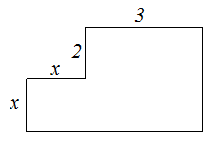
\includegraphics{capitulos/equacoes_de_primeiro_e_segundo_grau/media/image3.png}
\end{figure}

	\item{ Invente uma equação de 2º grau tal que o discriminante seja nulo.}

	\item{ Invente uma equação de 2º grau tal que:}

\begin{enumerate}[label=\alph*)]
	\item As soluções sejam reais e idênticas

	\item As soluções não sejam reais (complexas)

	\item As soluções sejam reais e distintas
\end{enumerate}

	\exitem{~ Resolva as equações usando qualquer método:}

a)~~ \textit{x(x-1)+3(x\textsuperscript{2}-1) = 0\quad \quad }\quad c)  \textit{(x+1)\textsuperscript{2} +(x – 1)\textsuperscript{ 2} = 0}

b)~~ \textit{2x(x-4)+2(x-1)= 0\quad \quad }\quad d) \textit{(x+2)\textsuperscript{ 2} + 2(x+1/2)\textsuperscript{ 2}= 0}

\end{exercicios}

\section{RESPOSTAS DOS EXERCÍCIOS PROPOSTOS}

\begin{respostas}{3}
	\ansitem{a) \textit{x = 4/3\quad \quad }}

	b) Até poderia ser usada a estratégia, porém somente após realizar a adição do lado direito.

	\ansitem{ \( x=-\frac{1}{3} \)}

	\ansitem{a)  \( -2 \) \quad \quad b) 2\quad ~~ c) 1\quad  \quad d) -2\quad \quad e) 4/6}

    f)  \( -5 \) \quad \quad g) 3\quad ~~ h) 6\quad \quad i) -10\quad \quad j) 7/2\quad

	\ansitem{\textit{x = 2}.}

	\ansitem{a)  \( x=1 \) \quad ~~ b)  \( x=\frac{5}{22} \) \quad c)  \( x=\frac{1}{7} \) \quad d)  \( x=2/5 \) \quad e) \(  x=-\frac{7}{2} \) ~~ f) \textit{x = -3.}}

    \ansitem{a)  \( 2 \) \quad \quad b)  \( -\frac{4}{3} \) \quad \quad c)  \( \frac{8}{5} \)}

    \ansitem{ \( x=1cm \)}

	\ansitem{a)  \( x=1cm \) \quad \quad \quad b)  \( x=\frac{3}{2}cm \)}


    \ansitem{ \( x=\frac{1}{2} \);}
    \ansitem{Comprimento=\textit{100m} e largura=\textit{70m};}
    \ansitem{\textit{2cm, 4cm } e \textit{ 6 cm}.}

\end{respostas}

\begin{respostas}{4}
	\ansitem{Não pois sem o coeficiente \textit{A} a equação se torna de 1º grau. Os coeficientes \textit{B} e \textit{C} podem ser nulos.}

	\ansitem{a) sim, b) não, c) o valor de \textit{x} é solução da equação, d) o valor de \textit{x} não é solução da equação}

	\ansitem{ a)  \( x= \pm 4 \) \quad \quad \quad \quad \quad d)  \( x'=0;x"=8 \)}

    \quad b)  \( x'=0;x"=-2 \) \quad \quad \quad \quad e)  \( x'=0;x"=2 \)

    \quad c)  \( x= \pm 3  \) \quad \quad \quad \quad \quad f)  \( x=0 \)

	\ansitem{a) 8\quad \quad \quad \quad \quad d) 30}

    \quad b) 6\quad \quad \quad \quad \quad e) 16

    \quad c) 12\quad \quad \quad \quad \quad f) 36\quad

	\ansitem{a)  \( x^{'}=1;x"=-5 \) \quad \quad \quad d)  \( x^{'}=6;x"=6 \)}

    \quad b)  \( x^{'}=3;x"=-4 \) \quad \quad \quad e)  \( x= \pm \sqrt[]{\frac{41}{4}}+\frac{3}{2} \)

    \quad c)  \( x^{'}=10;x"=4 \) \quad \quad \quad f)  \( x=\frac{1 \pm \sqrt[]{7}}{3} \)

	\ansitem{a)  \( x^{'}=x"=-2 \) \quad \quad \quad d)  \( x^{'}=2;x"=5 \)}

    \quad b)  \( x^{'}=3;x"=-4 \) \quad \quad \quad e)  \( x^{'}=-3;x"=-7 \)

    \quad c)  \( x^{'}=-2;x"=5 \) \quad \quad \quad f)  \( x^{'}=-1;x"=2 \)

	\ansitem{a) O método é eficiente porque as raízes são inteiras.}

    b) O método do produto e soma não é eficiente pois as raízes não são inteiras.

    \ansitem{a)  \( x^{'}=4;x"=-2 \) \quad \quad \quad d)  \( \frac{1 \pm \sqrt[]{-23})}{4} \)}

    \quad b)  \( x^{'}=-\frac{1}{2};x"=-\frac{1}{2} \) \quad \quad \quad e)  \( x^{'}=-\frac{1}{2};x^{''}=-2 \)

    \quad c)  \( x^{'}=1;~x"=6 \) \quad \quad \quad \quad f)  \( \frac{ \pm \sqrt[]{-32}}{2} \)

    \ansitem{ \( x \cong 0,4364 \)}

    \addtocounter{enumi}{2}
    \ansitem{a)  \( x^{'}=1;x"=0,75 \)}

    \quad b)  \( x^{'} \cong 3,302 \ldots ;~x" \cong -0,302 \ldots  \)

    \quad c)  \(  \pm \sqrt[]{-1} \)

    \quad d)  \( \frac{-2 \pm \sqrt[]{-2}}{2} \)

\end{respostas}